\documentclass[12pt, a4paper]{article}

\usepackage{array}
\usepackage[portuguese]{babel}
\usepackage{float}
\usepackage[a4paper, margin=2cm]{geometry}
\usepackage{graphicx}
\usepackage{hyperref}
\usepackage{pdfpages}
\usepackage{setspace}

\chardef\_=`_

\title{\textbf{Programação Orientada aos Objetos \\ \large Trabalho Prático}}
\date{12 de Maio 2024}
\author{Grupo TP32}

\begin{document}

\onehalfspacing
\setlength{\parskip}{\baselineskip}
\setlength{\parindent}{0pt}
\def\arraystretch{1.5}

\maketitle

\vspace{8cm}
\begin{center}
    \begin{tabular}{>{\centering}p{0.25\textwidth}
                    >{\centering}p{0.25\textwidth}
                    >{\centering\arraybackslash}p{0.25\textwidth}}
        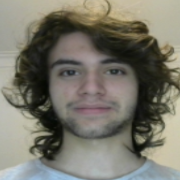
\includegraphics[width=4cm]{Diogo.jpeg}    &
        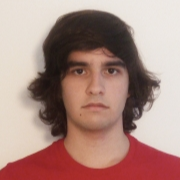
\includegraphics[width=4cm]{Humberto.jpeg} &
        
\includegraphics[width=4cm]{Jose.jpeg}     \\

        Diogo Costa & Humberto Gomes & José Lopes  \\
        A100751     & A104348        & A104541
    \end{tabular}
\end{center}
\pagebreak

\begin{abstract}
    No âmbito da Unidade Curricular de Programação Orientada aos Objetos, o nosso grupo desenvolveu
    uma aplicação de gestão de utilizadores, atividades e planos de treino. A aplicação permite a
    gestão destas entidades: criação tanto de novos utilizadores como de novas atividades, e
    associação de atividades a utilizadores como execuções individuais ou como parte de um plano de
    treino. Ademais, a aplicação permite a simulação da passagem do tempo para identificação das
    atividades como concluídas ou não, e permite a execução de interrogações sobre recordes (por
    exemplo, do maior número de calorias dispendido por um utilizador). Por último, foi implementado
    o conceito de atividade \emph{hard}, que de momento apenas é usado para caracterização de
    atividades na interface de linha de comandos desenvolvida, mas que pode vir a ser utilizado na
    expansão do programa.
\end{abstract}

\section{Arquitetura de classes}

Nesta secção, é descrita e justificada a arquitetura de classes da aplicação desenvolvida. Um
diagrama de classes pode encontrar-se no final deste documento.

\subsection{Entidades da aplicação}

Em primeiro lugar, abordar-se-ão as hierarquias de classes utilizadas para a representação das
entidades da aplicação. Todos os utilizadores são compostos pelos mesmos campos, mas podem
apresentar diferentes multiplicadores de calorias conforme o seu tipo (principiante, intermédio ou
avançado). Logo, a decisão arquitetural lógica foi o uso de uma classe abstrata para a representação
de um utilizador qualquer, \texttt{User}, que contém todas as variáveis de instância de um
utilizador. Não é permitida a instanciação de utilizadores sem conhecimento da sua experiência, pelo
que a cada nível de experiência está associada uma classe concreta (\texttt{BeginnerUser},
\texttt{IntermediateUser} ou \texttt{AdvancedUser}), que é subclasse de \texttt{User} e que
implementa o cálculo do multiplicador de calorias.

Para a implementação das atividades, foi utilizado um padrão arquitetural semelhante ao dos
utilizadores. A classe abstrata \texttt{Activity}, no topo da hierarquia, é responsável pelas
variáveis de instância comuns a todas as atividades (por exemplo, data de execução e duração). Na
base da hierarquia, estão as implementações de atividades em concreto, como levamento de pesos
(\texttt{ActivityWeightLifting}). No entanto, ao contrário do que ocorre com os utilizadores, há
certas variáveis de instância comuns a apenas algumas atividades (por exemplo, um número de
repetições). Logo, cada tipo de atividade que envolva o conhecimento de mais dados dá origem a uma
classe abstrata que herda de \texttt{Activity}, como ocorre com \texttt{ActivityRepetition}. Esta
classe poderá ter outras subclasses, algumas delas implementações de atividades (como
\texttt{ActivityPushUp}) e outras também tipos de atividades. Estes subtipos, como
\texttt{ActivityRepetitionWeighted}, envolvem as mesmas variáveis de instância que o tipo associado
à sua classe-pai, mas também outros dados que estarão presentes em todas as atividades do subtipo,
as suas subclasses. As atividades \emph{hard} são implementadas com recurso a uma interface vazia,
\texttt{ActivityHard}. Verificar se uma instância de atividade é difícil (por exemplo, para a
construção de um plano de treino) é tão simples como utilizar o operador \texttt{instanceof}.

Para compreender como as atividades são associadas a utilizadores, é necessário ter em conta a
interpretação do enunciado feita pelo nosso grupo. Considerou-se que uma instância de atividade é
executada a uma dada hora por um único utilizador, e que atividades não são identificáveis sem
estarem associadas ao seu utilizador. Também os planos de treino foram considerados entidades
fracas, associados a apenas um utilizador. Logo, utilizou-se uma estratégia de composição, onde
cada utilizador é dono do seu plano de treino e das suas atividades.

Um plano de treino, implementado em \texttt{TrainingPlan}, é uma coleção de atividades, que podem
ser repetidas várias vezes consecutivamente. Também é constituído pelo conjunto de dias da semana
em que é executado. A associação entre atividades e o seu número de execuções é feita através de um
mapeamento onde a chave é uma atividade, algo que é possível \footnote{\texttt{Activity} implementa
\texttt{hashCode} e \texttt{equals}, e \texttt{TrainingPlan} garante que atividades não são
modificadas sem reinserção no \texttt{Map}.} mas que dificulta a leitura do diagrama de classes UML.
Planos de treino garantem a não-sobreposição de atividades e expõem métodos úteis para verificar o
mesmo para atividades externas. Ademais, implementam a construção do conjunto de atividades entre
duas datas resultantes da sua execução.

A coleção de atividades de um utilizador, \texttt{UserActivities}, foi separada da classe
\texttt{User} que a contém, de modo a respeitar o princípio da responsabilidade única: o utilizador
não deve conter a lógica de gestão da sua coleção de atividades. Esta coleção contém um plano de
treino e dois conjuntos de atividades, as concluídas e não concluídas. Instâncias desta classe são
responsáveis pela movimentação de atividades por concluir para o conjunto de atividades concluídas,
quando se lhes passa uma mensagem de avanço de tempo.

Por fim, a classe \texttt{FitnessModel} contém todos os dados da aplicação, um mapa entre códigos
identificadores de utilizadores e os utilizadores em si, que por sua vez contêm, através de
\texttt{TrainingPlan} e \texttt{UserActivities}, as atividades existentes. Todas as classes
mencionadas até este momento implementam a interface \texttt{java.io.Serializable}, permitindo o
armazenamento persistente do estado da aplicação através da serialização da instância de
\texttt{FitnessModel}.

\subsection{Interrogações}

As interrogações sobre recordes de atividades são todas implementações da interface funcional
\texttt{java.util.function.Consumer<User>}. \texttt{FitnessModel}, durante a execução de uma destas
\emph{queries}, itera pelos utilizadores da aplicação, que são consumidos pela instância da
interrogação. No final, poder-se-ão enviar mensagens a esta para se conhecer o resultado calculado.
Como algumas destas interrogações envolvem restrições entre duas datas, criou-se a classe abstracta
\texttt{QueryBetweenDates}, que gere este intervalo de datas e fornece um método às suas subclasses,
implementações de \emph{queries}, para a determinação de se uma dada atividade cumpre os requisitos
do filtro de datas existente. A única interrogação que não se encaixa na descrição providenciada é
\texttt{QueryDistance}, também um \texttt{Consumer<User>} mas que tem em conta um utilizador apenas.
Segue-se a associação entre as classes das interrogações e as suas funcionalidades:

\begin{itemize}
    \item \texttt{QueryDistance} -- Cálculo da distância percorrida por um utilizador;
    \item \texttt{QueryHardestTrainingPlan} -- Determinação do plano de treino que exige o dispêndio
        de mais calorias (por semana);
    \item \texttt{QueryMostActivities} -- Determinação do utilizador que realizou o maior número de
        atividades;
    \item \texttt{QueryMostCalories} -- Determinação do utilizador que dispendeu o maior número de
        calorias;
    \item \texttt{QueryMostCommonActivity} -- Determinação da classe de atividade mais executada.
\end{itemize}

\subsection{Exceções}

Foram definidos vários tipos de exceção, para se poder gerir o fluxo de controlo no caso de
ocorrerem erros. Por exemplo, quando valores inválidos são providenciados a construtores e a
\emph{setters} de utilizadores, estes podem levantar uma \texttt{UserException}. O mesmo se tem para
atividades e \texttt{ActivityException}. As exceções \texttt{ActivityDoesntExistException} e
\texttt{ActivityOverlapException} têm nomes auto-descritivos e são levantadas na inserção e remoção
de atividades, respetivamente, ambas em planos de treino e coleções de atividades de um utilizador.
Por último, \texttt{FitnessModelException} é levantada para os diversos erros de interação com
\texttt{FitnessModel}, e \texttt{FitnessControllerException} é uma exceção utilizada para a vista
da interface com o utilizador não aceder aos tipos de exceção do modelo, sendo todas as exceções
vindas do modelo recriadas pelo controlador (a arquitetura \emph{Model-View-Controller} será
descrita de seguida). Optou-se por não se criar uma classe base para exceções da aplicação
\emph{Fitness}, para desencorajar os desenvolvedores a não distinguirem entre os diferentes tipos de
erro.

\subsection{Interação com o utilizador}

A interação com o utilizador foi implementada de acordo com o padrão de conceção MVC
\emph{Model-View-Controller}. \texttt{FitnessModel}, classe já apresentada, contém os dados da
aplicação, enquanto que \texttt{FitnessController} constitui um adaptador entre
\texttt{FitnessModel} e \texttt{FitnessView}, a interface com o utilizador, desacoplando assim o
modelo da interface com o utilizador. Algumas classes auxiliares foram criadas para suportar a
vista: \texttt{Menu} e \texttt{MenuEntry}, um menu formado por entradas compostas por uma
\texttt{String} e um \emph{handler} que é chamado quando essa opção é escolhida, e
\texttt{UserInput}, um \emph{wrapper} de um \texttt{java.util.Scanner} que permite uma leitura da
entrada do utilizador resiliente a erros.

Foram utilizadas capacidades de reflexão da linguagem Java para simplificar a implementação do
controlador e da vista, o que também facilita a adição de novos utilizadores, atividades e
interrogações. Por exemplo, o controlador expõe à vista o nome das classes dos utilizadores
disponíveis. Após ler todos os campos necessários, a vista passará, juntamente com o nome da classe
escolhida, a informação lida ao controlador, que criará o utilizador do tipo correto e o adicionará
ao modelo. A implementação da entrada de atividades é um pouco mais complexa, pois exige dar a
conhecer à vista que outros campos têm de ser pedidos ao utilizador. Mesmo assim, julgamos que esta
solução é menos extensa do que a enumeração de tipos de atividade na vista. Com o uso de reflexão, a
expansão do programa torna-se muito simples: para a criação de um novo tipo de utilizador ou de uma
nova atividade de um tipo existente, além da criação da nova classe, é apenas necessária a inserção
de uma linha de código em \texttt{FitnessController}, a adição da classe criada à lista de classes
conhecidas.

\section{Descrição da aplicação}

Após transferir o repositório \texttt{git}, a aplicação pode ser executada com o comando
\texttt{gradle run}. Em alternativa, pode correr-se a aplicação externamente após a sua compilação,
evitando a elevada latência adicionada pelo redirecionador de I/O do \texttt{gradle}:

\begin{center}
    \texttt{gradle build \&\& unzip build/distributions/poo.zip \&\& ./poo/bin/poo}
\end{center}

Após correr o comando anterior, o utilizador deparar-se-á com o seguinte menu: \\

\begin{figure}[H]
    \centering
    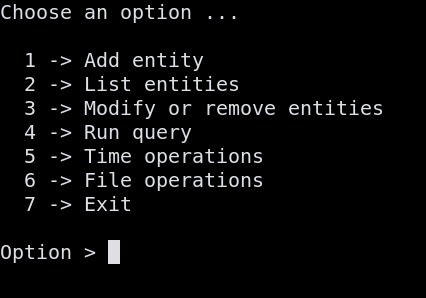
\includegraphics[width=0.4\textwidth]{MainMenu.png}
    \caption{Menu principal da aplicação.}
\end{figure}

Para adicionar uma nova entidade, a opção 1 é escolhida, e o utilizador pode escolher entre
adicionar um novo utilizador ou uma nova atividade, como se vê na figura abaixo. Enquanto não forem
adicionados utilizadores, não é possível adicionar atividades, como informaria uma mensagem de erro
caso essa opção fosse escolhida. Segue-se um exemplo do que ocorre quando se opta por inserir um
utilizador. \\

\begin{figure}[H]
    \centering
    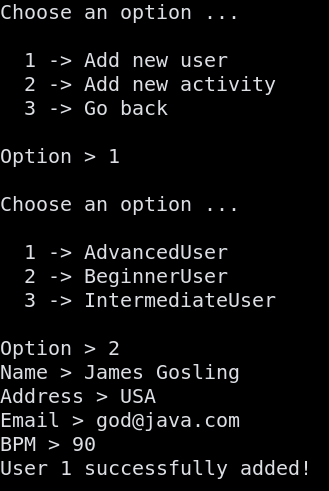
\includegraphics[width=0.35\textwidth]{NewUser.png}
    \caption{Inserção de um novo utilizador.}
\end{figure}

Como se observa, primeiro é pedido o tipo do utilizador e depois o valor dos seus campos. Segue-se
uma mensagem com o identificador do novo utilizador criado.

Podem agora inserir-se novas atividades. Estas podem ser eventos isolados ou parte do plano de
treino do utilizador providenciado, informação que a aplicação pede, como se observa na figura
abaixo. Depois, serão pedidos os valores dos atributos necessários conforme o tipo de atividade
escolhido. \\

\begin{figure}[H]
    \centering
    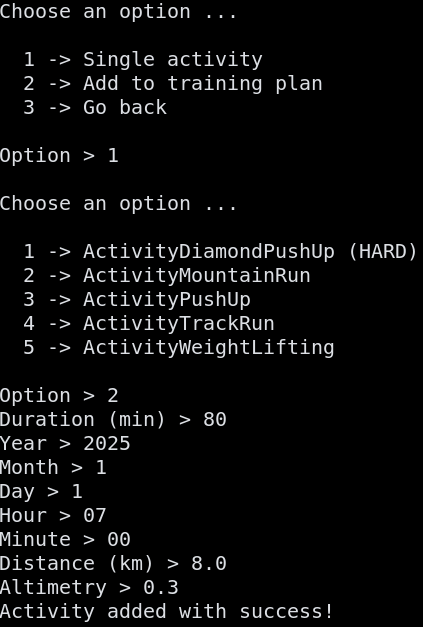
\includegraphics[width=0.4\textwidth]{NewActivity.png}
    \caption{Inserção de uma nova atividade.}
\end{figure}

Os vários utilizadores e as várias atividades podem ser consultados escolhendo a opção 2 no menu
principal. Note-se que as atividades têm de ser filtradas conforme o seu estado de conclusão ou a
sua pertença a um plano de treino. \\

\begin{figure}[H]
    \centering
    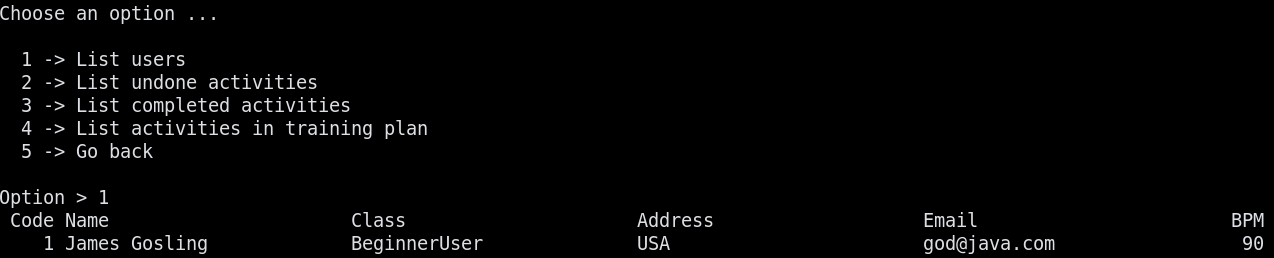
\includegraphics[width=\textwidth]{ListUsers.png}
    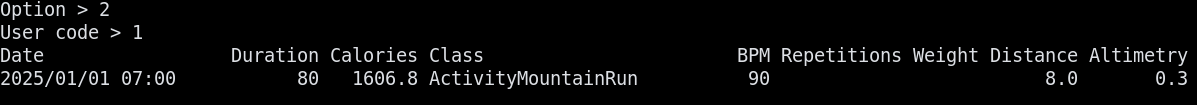
\includegraphics[width=\textwidth]{ListActivities.png}
    \caption{Enumeração de utilizadores e de atividades.}
\end{figure}

A opção 3 do menu principal permite a remoção de utilizadores e a modificação dos dias em que planos
de treino são executados. Exemplifica-se esta segunda operação na figura abaixo, onde a aplicação
pede o código do utilizador e os dias de execução um a um: \\

\begin{figure}[H]
    \centering
    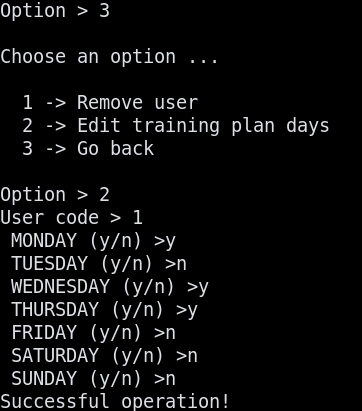
\includegraphics[width=0.35\textwidth]{EditTrainingPlan.png}
    \caption{Edição dos dias de execução de um plano de treino.}
\end{figure}

A opção 4 do menu principal permite a execução de uma \emph{query}. É pedida ao utilizador a
interrogação que deve ser executada, seguida dos argumentos necessários para a sua parametrização.
Segue-se o exemplo da consulta da atividade mais comum, que não requer qualquer argumento. Note-se
que nenhuma atividade será encontrada, pois esta interrogação apenas contabiliza atividades já
executadas. \\

\begin{figure}[H]
    \centering
    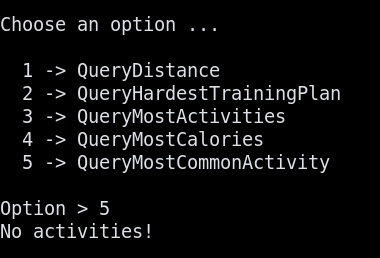
\includegraphics[width=0.4\textwidth]{RunQuery.png}
    \caption{Execução de uma interrogação.}
\end{figure}

Se seguida, a opção 5 do menu principal permite consultar o tempo atual na aplicação e avançar o
tempo, operação que é vista na figura abaixo. \\

\begin{figure}[H]
    \centering
    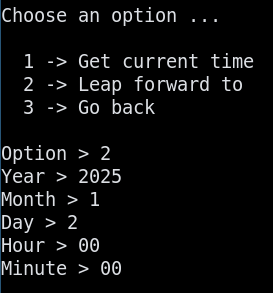
\includegraphics[width=0.3\textwidth]{LeapForward.png}
    \caption{Avanço do tempo para uma data posterior.}
\end{figure}

Agora, caso o utilizador repita a \emph{query} executada anteriormente, poderá verificar que, como a
única atividade criada já foi executada, a atividade mais frequente será, com uma única execução,
\texttt{ActivityMountainRun}.

Por último, podem realizar-se operações como leituras e escritas para ficheiro. Após se escolher um
caminho de ficheiro, o programa a serializa o estado da aplicação e a armazena-o com sucesso.
Este ficheiro pode ser depois lido e o estado da aplicação restaurado. \\

\begin{figure}[H]
    \centering
    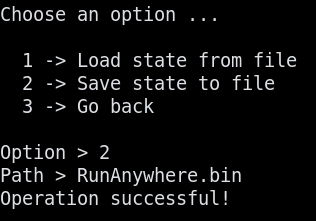
\includegraphics[width=0.35\textwidth]{SaveFile.png}
    \caption{Serialização do estado da aplicação para ficheiro.}
\end{figure}

\section{Conclusão}

Em suma, o nosso grupo foi capaz de desenvolver a aplicação proposta, cumprindo a maioria dos
requisitos, para ser específico, os requisitos para a nota máxima de 18 valores. O leitor pode
questionar-se por que motivo o nosso grupo não conseguiu cumprir a totalidade dos requisitos.

A complexidade do projeto proposto não é elevada, e o nosso grupo não sentiu dificuldades na
implementação da funcionalidade pedida. No entanto, a maioria das dificuldades encontradas têm
origem numa única característica da linguagem Java: a sua verbosidade. A implementação de cada
funcionalidade tomou muito mais do nosso tempo do que o esperado, devido à quantidade de código que
era necessário escrever. A título de exemplo, o comportamento de cada interrogação é definido por
apenas um método, mas a criação de cada interrogação exige também a definição de vários
construtores, \emph{getters}, e métodos como \texttt{equals} e \texttt{clone}. Este maior esforço
necessário não era esperado, conduzindo a um atraso no desenvolvimento que impediu a realização do
último dos requisitos. Por outro lado, esta verbosidade é o que torna o código Java extremamente
legível, pelo que esta característica da linguagem é definitivamente uma espada de dois gumes.

No entanto, considerando apenas os requisitos implementados, o nosso grupo encontra-se
satisfeito com o resultado produzido: uma aplicação modular, que respeita os princípios do
encapsulamento, facilmente extensível, que faz uso de mecanismos de reutilização de código,
fartamente documentada e extensivamente testada.


\includepdf[pages=-,fitpaper=false,angle=90]{ProjectDiagram/UMLDiagram.pdf}

\end{document}
